%!TEX encoding = IsoLatin
%!TEX main = ../../main.tex

\section{Self-Sovereign-Identity as a Service}
The idea of a Self-Sovereign-Identity as a Service is to support a constrained device to create and manage its self-sovereign-identity. Since IoT devices cannot run natively the complete SSI stack there is a need to design and develop an edge device capable of providing such an identity to constraint devices as a service.  Such a solution has the advantage of increasing the number of devices that can interact in such a secure digital ecosystem.

\subsection{Use case analysis}
The first step is to analyse and identify critical cryptographic operations involved in self-sovereign-identity management.The examples in figures \ref{usecase-did}, \ref{usecase-issuer} and \ref{usecase-verifier} illustrate in an high-level way how to create and use verifiable credentials. 
\begin{figure}[!h]
    \centering
    \includesvg[inkscapelatex=false, scale=0.80]{./chapters/images/use-case-did_creation.svg}
    \caption{Creation of a DID}
    \label{usecase-did}
\end{figure}

Independently from the chosen registry when a holder creates a DID, he uniquely binds cryptographic proofs with the DID identifier, typically using public-private key pairs, so he will need to generate them before generating the DID document. The order of operations can be seen in figure \ref{usecase-did}. 

\begin{figure}[!h]
    \centering
    \includesvg[inkscapelatex=false, scale=0.80]{./chapters/images/use-case-credential_creation.svg}
    \caption{Issuance - verifiable credential creation}
    \label{usecase-issuer}
\end{figure}
Next, a holder can get a verifiable credential from an issuer, that will verify the identity in some way, by examining the provided documentation, if the requirements are satisfied the issuer will generate a verifiable credential by linking her identity information to DID. The holder receiving the verifiable credential will verify its validity and save it in his personal credential repository. All of this is shown in figure \ref{usecase-issuer}. 

\begin{figure}[!h]
    \centering
    \includesvg[inkscapelatex=false, scale=0.80]{./chapters/images/use-case-credential_usage.svg}
    \caption{Verification - verifiable credential usage}
    \label{usecase-verifier}
\end{figure}

Moreover, as can be seen in figure \ref{usecase-verifier}, once a holder has a DID and a verifiable credential, he can use them to access a service to a verifier. The holder will use the DID to prove to the requesting party that it is the controller of that DID through some sort of challenge-response. Then the holder, starting from one or more verifiable credentials will create a verifiable presentation. If possible it is recommended to the holder use selective disclosure, presenting proofs of claims without revealing the entire verifiable credential. Once created the verifiable presentation the holder can send it to the verifier and he will check its validity and authorize the holder if everything is fine.  
After analysing the different use cases, as highlighted in figures \ref{usecase-did}, \ref{usecase-issuer} and \ref{usecase-verifier}, the cryptographic operations that could be  critical for a constrained device are:
\begin{itemize}
    \item keys generation
    \item signature generation and verification
    \item proof generation and verification
\end{itemize}

To understand how much critical these operations are on a constrained device it is necessary to analyse the differences between a non-constrained one by getting their execution times and comparing the result. 
STM32L4+ Discovery kit IoT node\cite{stm32-board-product} has been used as a constrained device equipped with the \texttt{STM32L4S5 MCU @ 120 MHz}, 2 Mbytes of flash memory and 640 Kbytes of SRAM. While, as a non-constrained device, which has also been called \textit{edge device}, has been used a server with an \texttt{Intel Xeon Silver 4110 CPU @ 2.10GHz}. As a library that implements the operation for key generation and signature (generation and verification), Mbed TLS has been used. \textit{Mbed TLS} is a C library that implements cryptographic primitives, it supports RSA, ECDSA, and other algorithms such as Ed25519. It has a small code footprint which makes it reasonable to use for embedded systems \cite{mbed-tls}. To test if a constrained device could be capable to implement and use some \textit{zero-knowledge proof} mechanisms, it has been decided to use a library which implements the BBS\texttt{+} signature scheme \cite{bbsplus}. BBS\texttt{+} signatures can be used to generate signature proofs of knowledge and selective disclosure zero-knowledge proofs \cite{bbs-rust} and they are implemented on top of BLS12-381 elliptic curve \cite{bls-curve}, which is a curve not supported in Mbed TLS. Since available BBS\texttt{+} libraries are also not supported for STM32L4, it has been decided to take execution times only on the edge device. Then execution times between the ECDSA signature scheme and BBS\texttt{+} signature scheme are comparable since they are been taken on the same architecture and they are both elliptic curve signature schemes.

\begin{figure}[h!]
    \centering
    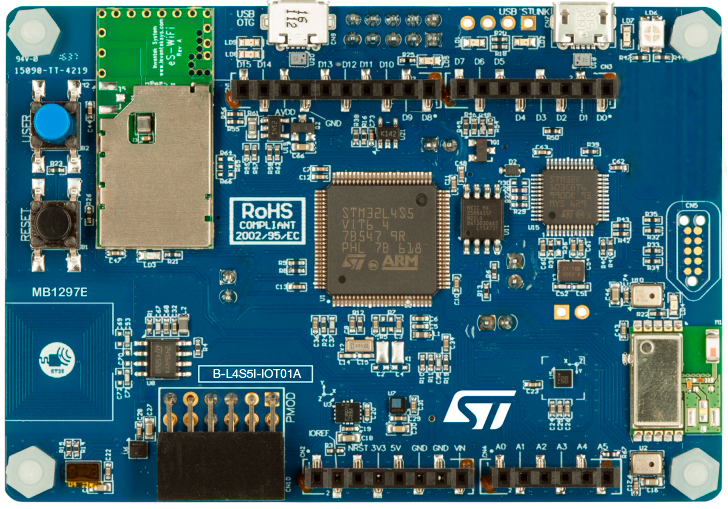
\includegraphics[scale=0.30]{./chapters/images/STM32L4+ Discovery kit IoT node.jpeg}
    \caption{STM32L4+ Discovery kit IoT node\cite{stm32-board-product}.}
    \label{stm-board}
\end{figure}

\subsubsection*{Results}
It is evident from the table \ref{time-table1} that RSA is usable on constrained devices in real-life applications only if the key generation is precomputed, otherwise is unusable. On the constrained device, RSA signing and verification are faster than ECDSA, but ECDSA provides the same level of security as RSA but it does so while using much shorter key lengths. In applications where it could be useful to generate a keypair on the fly, ECDSA is a must. On the edge device, the ECDSA signing operation is faster than RSA, while the RSA verification process is faster than ECDSA.  It can also be noted that the time difference between the constrained device and the edge device is huge, probably due to the frequency of operation of the MCU and the CPU.

\begin{table}[!h]
    \centering
    \begin{tabular}{| l || r | r | r |}
        \hline      
        \textbf{Operation} & \textbf{constrained device}$^\star$ & \textbf{edge device}$^\star$ \\ [0.5ex] 
        \hline \hline 
        EC-p256-keygen                  & 318 ms  & 0.5 ms \\
        \hline
        ECDSA-p256-SHA256-sign          & 1\,503 ms & 0.6 ms \\
        \hline
        ECDSA-p256-SHA256-ver           & 6\,031 ms & 2.0 ms \\
        \hline \hline
        RSA2048-keygen                  & 622\,749 ms  & 186  ms \\
        \hline
        RSA2048-SHA256-sign          & 1\,305 ms & 3.60 ms \\
        \hline
        RSA2048-SHA256-ver           & 331 ms & 0.07  ms \\
        \hline
    \end{tabular}\\
    \footnotesize $^\star$mbedTLS library
    \caption{Execution time comparison between constrained and non-constrained devices}
    \label{time-table1}
\end{table}

Furthermore, in table \ref{time-table2} ECDSA signatures and BBS\texttt{+} signatures are compared on the same CPU architecture. The obtained results are that BBS\texttt{+} signature scheme is much slower than the ECDSA one, even if they are both elliptic curve based. The order of magnitude of the percentage increase is 3, which is a significant difference. 
   
\begin{table}[!h]
    \centering
    \begin{tabular}{| l || r | r | r|}
        \hline 
        \textbf{Operation} & \textbf{ECDSA}$^\star$ & \textbf{BBS\texttt{+}}$^\star$$^\dagger$ & \textbf{\% increase} \\ [0.5ex] 
        \hline  \hline 
        keygen   & 0.2   ms      & 39 ms   &\texttt{+}7\,800\\
        \hline
        sign     & 0.6   ms      & 27  ms   &\texttt{+}4\,500\\
        \hline
        verify   & 2.0  ms         & 166 ms   &\texttt{+}8\,300\\
        \hline
    \end{tabular}
    \\
    \footnotesize $^\star$Xeon 2.10GHz \enspace\enspace $^\dagger$Rust bbs library
    \caption{Execution time comparison between ECDSA and BBS\texttt{+}}
    \label{time-table2}
\end{table}

\subsection{Design and implementation choices}
The obtained results suggest that a constrained device cannot use the BBS\texttt{+} signature scheme in real-world applications, since it can be supposed that execution times will be considerably high. In the Self-sovereign Identity as a Service (SSIaaS) paradigm, a new role is defined, called edge. The edge device interacts with a constrained IoT object and provides functionalities to create and support it in identity management, this can be seen in figure \ref{poc-design}. The identified and exposed operations by the edge device are:
\begin{itemize}
    \item key pairs generation
    \item storage of a verifiable credential
    \item generation of a verifiable presentation
\end{itemize}

{\color{red} ToDo: spiegare il design delle operazioni}
\begin{figure}[!h]
    \centering
    \includesvg[inkscapelatex=false, scale=1]{./chapters/images/poc.svg}
    \caption{Basic components of Self-Sovereign-Identity as a Service}
    \label{poc-design}
\end{figure}

\begin{figure}[!h]
    \centering
    \includesvg[inkscapelatex=false, scale=0.7]{./chapters/images/poc_gen_keys.svg}
    \caption{Key pairs generation operation in detail}
    \label{poc-gen-keys}
\end{figure}

\begin{figure}[!h]
    \centering
    \includesvg[inkscapelatex=false, scale=0.7]{./chapters/images/poc_store_vc.svg}
    \caption{Storage of a verifiable credential operation in detail}
    \label{poc-store-vc}
\end{figure}

\begin{figure}[!h]
    \centering
    \includesvg[inkscapelatex=false, scale=0.7]{./chapters/images/poc_get_vp.svg}
    \caption{Generation of a verifiable presentation operation in detail}
    \label{poc-get-vp}
\end{figure}

\subsection{Architecture}
{\color{red} ToDo: spiegare provisioning iniziale e architettura finale}
\begin{figure}[!h]
    \centering
    \includesvg[inkscapelatex=false, scale=0.7]{./chapters/images/manufacturer.svg}
    \caption{Manufacturer provisions device with expected hashes, keys and signature of the public key}
    \label{manufacturer-provisioning}
\end{figure}

\begin{figure}[!h]
    \centering
    \includesvg[inkscapelatex=false, scale=0.7]{./chapters/images/Demo architecture3.svg}
    \caption{Demo architecture}
    \label{poc-architecture}
\end{figure}
